\documentclass[border=4pt]{standalone}
\usepackage{amsmath,amssymb,tikz}
\usetikzlibrary{arrows.meta}
\definecolor{figB}{RGB}{31,90,166}\definecolor{figR}{RGB}{176,48,48}\definecolor{figG}{RGB}{46,125,50}\definecolor{figO}{RGB}{214,120,20}
\begin{document}
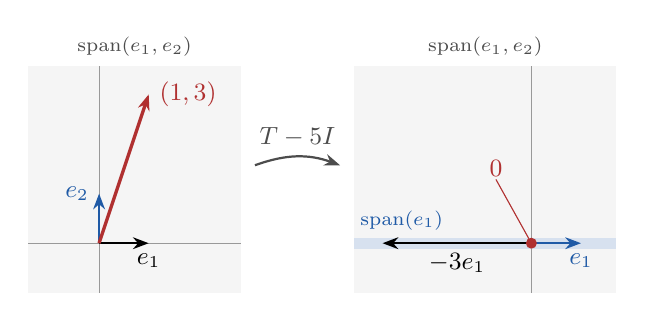
\begin{tikzpicture}[scale=0.9,>={Stealth[length=2mm]}]
% domain: the plane span(e1,e2)
\fill[black!4] (-1.0,-0.7) rectangle (2.0,2.5);
\node[font=\scriptsize,black!70,above] at (0.5,2.5) {$\operatorname{span}(e_1,e_2)$};
\draw[thin,black!40] (-1.0,0)--(2.0,0); \draw[thin,black!40] (0,-0.7)--(0,2.5);
\draw[->,thick] (0,0)--(0.7,0) node[below,font=\small]{$e_1$};
\draw[->,thick,figB] (0,0)--(0,0.7) node[left,font=\small]{$e_2$};
\draw[->,very thick,figR] (0,0)--(0.7,2.1) node[right,font=\small]{$(1,3)$};
% the map
\draw[->,thick,black!70] (2.2,1.1) to[bend left=20] node[above,font=\small]{$T-5I$} (3.4,1.1);
% target: everything lands in the line span(e1)
\begin{scope}[xshift=6.1cm]
\fill[black!4] (-2.5,-0.7) rectangle (1.2,2.5);
\node[font=\scriptsize,black!70,above] at (-0.65,2.5) {$\operatorname{span}(e_1,e_2)$};
\draw[thin,black!40] (0,-0.7)--(0,2.5);
\draw[line width=4pt,figB!18] (-2.5,0)--(1.2,0);
\node[font=\scriptsize,figB,above right,inner sep=2pt] at (-2.5,0.1) {$\operatorname{span}(e_1)$};
\draw[->,thick] (0,0)--(-2.1,0) node[pos=0.5,below,font=\small]{$-3e_1$};
\draw[->,thick,figB] (0,0)--(0.7,0) node[below,font=\small]{$e_1$};
\fill[figR] (0,0) circle (2.2pt);
\draw[figR,thin] (0,0)--(-0.5,0.9) node[above,font=\small,figR,inner sep=1pt]{$0$};
\end{scope}
\end{tikzpicture}
\end{document}
